\definecolor{lightgray}{HTML}{dddddd}
\definecolor{medgray}{HTML}{cccccc}
\definecolor{medgray2}{HTML}{bbbbbb}
\definecolor{darkgray}{HTML}{999999}
\definecolor{lightgp}{HTML}{ddddee}
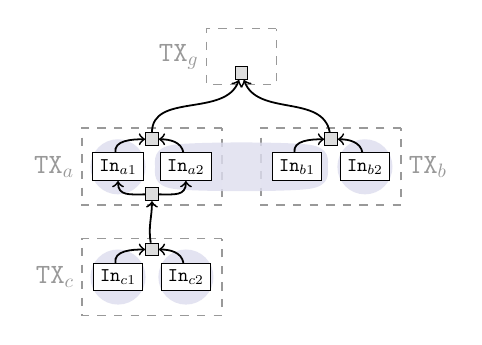
\begin{tikzpicture}[x=1.12cm, scale=0.7, every node/.append style={transform shape}]
    \begin{scope}[all/.style={draw,fill=white,minimum height=0.5cm, minimum width=0.5cm},line width=0.08ex]
    \begin{scope}[color=darkgray,dashed,line width=0.2ex]
        \node[all, label={[anchor=east, font=\fontsize{14}{14}]left:$\texttt{TX}_g$},
        rectangle,minimum width=0.5in, minimum height=0.4in, line width=0.15ex] (a0) at (0, 0) {};
        \node[all, label={[anchor=east, font=\fontsize{14}{14}]left:$\texttt{TX}_a$}, rectangle,minimum width=1in, minimum height=0.55in, line width=0.15ex]
        (a1) at (-1.45, -2) {};
        \node[all, label={[anchor=west, font=\fontsize{14}{14}]right:$\texttt{TX}_b$}, rectangle,minimum width=1in, minimum height=0.55in, line width=0.15ex]
        (a2) at (1.45, -2) {};
        \node[all, label={[anchor=east, font=\fontsize{14}{14}]left:$\texttt{TX}_c$}, rectangle,minimum width=1in, minimum height=0.55in, line width=0.15ex]
        (a3) at (-1.45, -4) {};
    \end{scope}
    
        \node[fill=lightgp, circle,minimum width=1cm, opacity=0.8] (pt1) at (-2, -2) {};
        \node[fill=lightgp, circle,minimum width=1cm, opacity=0.8] (pt4) at (2, -2) {};
        \node[fill=lightgp, circle,minimum width=1cm, opacity=0.8] (pt5) at (-2, -4) {};
        \node[fill=lightgp, circle,minimum width=1cm, opacity=0.8] (pt6) at (-0.9, -4) {};
        \fill[color=lightgp, opacity=0.8] plot[smooth cycle] coordinates { (1.4, -2) (1.1, -2.4) (-1.1, -2.4) (-1.4, -2) (-1.1, -1.6) (1.1, -1.6)} node (pt2) {};
        %\fill[color=lightgp] plot[smooth cycle] coordinates {(2.1, -1.75) (2, -2.4) (0.6, -3.4) (0, -3.5) (-0.3, -3.3)(-0.3, -2.8) (0.1, -2.4) (1.2, -1.65) (1.7, -1.5) } node (pt3) {};
        
        \node[rectangle, fill=lightgray, draw, minimum width=1ex](ain) at (-1.45, -1.5) {};
        \node[rectangle, fill=lightgray, draw, minimum width=1ex](bin) at (1.45, -1.5) {};
        \node[rectangle, fill=lightgray, draw, minimum width=1ex](aout) at (-1.45, -2.5) {};
        \node[rectangle, fill=lightgray, draw, minimum width=1ex](cin) at (-1.45, -3.5) {};
        \node[rectangle, fill=lightgray, draw, minimum width=1ex](gout) at (0, -0.3) {};
        
        %\node[all, draw] (b0) at (0, 0) {$\texttt{In}_a$};
        \node[all, draw] (b1) at (-2, -2) {$\texttt{In}_{a1}$};
        \node[all, draw] (b2) at (-0.9, -2) {$\texttt{In}_{a2}$};
        \node[all, draw] (b3) at (0.9, -2) {$\texttt{In}_{b1}$};
        \node[all, draw] (b4) at (2, -2) {$\texttt{In}_{b2}$};
        
        \node[all, draw] (b5) at (-2, -4) {$\texttt{In}_{c1}$};
        \node[all, draw] (b6) at (-0.9, -4) {$\texttt{In}_{c2}$};
        
        \begin{scope}[line width=0.15ex]
        \path[->] (ain) edge[out=90, in=-110] node[sloped,above] {} (gout) ;
        \path[->] (bin) edge[out=100, in=-70] node[sloped,above] {} (gout) ;
        \path[->] (cin) edge[out=100, in=-90] node[sloped,above] {} (aout) ;
        \path[->] (b1) edge[out=100, in=180] node[sloped,above] {} (ain);
        \path[->] (b2) edge[out=100, in=0] node[sloped,above] {} (ain);
        \path[->] (b3) edge[out=100, in=180] node[sloped,above] {} (bin);
        \path[->] (b4) edge[out=100, in=0] node[sloped,above] {} (bin);
        \path[->] (b5) edge[out=100, in=180] node[sloped,above] {} (cin);
        \path[->] (b6) edge[out=100, in=0] node[sloped,above] {} (cin);
        \path[->] (aout) edge[out=180, in=-90, looseness=1.3] node[sloped,above] {} (b1);
        \path[->] (aout) edge[out=0, in=-90, looseness=1.3] node[sloped,above] {} (b2);
        \end{scope}
        %\node[] (p1) at (3, 0.5) {\footnotesize$\mathcal{P}_{T_1}$};
        %\node[] (p2) at (3, 0) {\footnotesize$\mathcal{P}_{T_2} = \mathcal{P}_{T_3}$};
        %\node[] (p3) at (3, -0.5) {\footnotesize$\mathcal{P}_{T_9} = \mathcal{P}_{T_6} = \mathcal{P}_{T_7}$};
        \begin{scope}[color=darkgray,dashed,line width=0.2ex]
        %\path[->] (p1) edge[out=180, in=0] node[sloped,above] {} (pt1) ;
        %\path[->] (p2) edge[out=180, in=60] node[sloped,above] {} (pt2) ;
        %\path[->] (p3) edge[out=-90, in=30] node[sloped,above] {} (pt3) ;
        \end{scope}
    \end{scope}
\end{tikzpicture}
